\section{Evaluation}
\label{sec:eval}

All results are modelled, and ratios above 1 favour CoDe.

\subsection{Methodology}
\label{sec:eval:method}

\subsubsection{Hardware platforms}
The mobile platform pairs the Snapdragon 8 Gen 3~\cite{sd8g3} host and NPU with PIM on LP-Spec's~\cite{lpspec} x64
LPDDR5-6400 (4 dies $\times$ 16 banks, 409.6\,GB/s internal). The NPU computes at 12\,TOPS, its measured FP16 GEMM rate~\cite{hao2025}
used for INT8\ASSUMPTION, and reads the memory at 42\,GB/s (Section~\ref{sec:bg:roofline}). Each host visit costs
30\,\textmu s of NPU dispatch~\cite{npufaster}\ASSUMPTION; the host draws 2.285\,W while busy, the 8 Gen 3's~\cite{sd8g3}
decode power net of its DRAM~\cite{hao2025,heterollm,tman}\ASSUMPTION. The edge server pairs P3-LLM's~\cite{p3llm} NPU with one
HBM2 stack of 16 pseudo-channels (1,024\,GB/s internal); the NPU idles at 55\,W, the chip idle power of
TPUv4i~\cite{tpuv4i}, while the PIM works\ASSUMPTION.

\subsubsection{PIM designs and area}
Each substrate carries four designs, stock AiM~\cite{aimjssc}, P3-LLM-style, LP-Spec-style and CoDe, with one
controller and the same PU placement (Table~\ref{tab:params}). Every design computes at its rival's
precision: INT8 on the mobile platform, as LP-Spec~\cite{lpspec} does, and W4A8 with a 4-bit KV cache on HBM2, as
P3-LLM~\cite{p3llm} does, with every design's arithmetic priced as INT4\,$\times$\,INT8 integers\ASSUMPTION. On the
mobile platform CoDe's tile of $V = 8$ spans two column periods, so one MAC command serves eight tokens. On HBM2 each
token's staging slice is twice as large and every PU serves two banks, so we set $V = D = 4$, the tile with the higher
throughput per logic mm$^2$ of the two tiles we evaluated there ($V = 4$ and 8). CoDe reaches LP-Spec-style's peak on
the mobile platform with 0.539$\times$ its logic area per die: arithmetic takes 0.73 of LP-Spec-style's logic and 0.34
of CoDe's, while storage, the staging register, accumulator file and weight latch, takes 0.32 of CoDe's logic and 0.10
of LP-Spec-style's. On HBM2, CoDe's logic is 0.56$\times$ LP-Spec-style's and 1.33$\times$ P3-LLM-style's, an area
that buys twice P3-LLM-style's beats per column.

\subsubsection{Simulator and models}
We extend the open-source trace-driven AiM simulator, built on Ramulator~2.0~\cite{ramulator2} and used by
CENT~\cite{cent}, with each design's commands and a PU model that holds a MAC command until the PU has finished the
beats of the previous command; every PIM kernel runs at cycle level. Our P3-LLM-style model reproduces
P3-LLM's~\cite{p3llm} own step gain of depth 2 over a depth-1 PIM: 1.78$\times$ at INT8 against the 1.6$\times$ P3-LLM
reports. On the mobile platform the simulator gives P3-LLM-style's per-token commands no separate C/A slot;
re-timed on the C/A bus, the commands lower P3-LLM-style's $U$ from 0.384 to 0.380, and on the edge server the
simulator times them. The mobile runs issue refreshes without their refresh cycle time, so refresh takes no share of
the mobile time ($\rho = 0$ in Section~\ref{sec:bg:cmd}). Area comes from synthesis of each PU's lanes and registers in a 45\,nm library, scaled to a 1z DRAM process by
the published area of AttAcc's~\cite{attacc} GEMV unit in that process; the GB is priced as DRAM-process
SRAM\ASSUMPTION. PU power and energy come from synthesis of each design's whole PU with Yosys and ABC~\cite{abc} on the
Nangate45 library, OpenROAD~\cite{openroad} placement and clock-tree synthesis, and OpenSTA power from a zero-delay
simulation with random operands. We scale the synthesised energy to the DRAM process so that an AiM-style bf16 PU from
the same flow spends the compute share of CENT's~\cite{cent} AiM MAC-command energy, and with the square of the voltage
to the 1.05\,V supply (VDD2H on LPDDR5); leakage scales the same way\ASSUMPTION. Peak power runs every PU at its full
MAC rate and includes leakage, GB reads and the column fetch, which adds 87.6\,mW per die on the mobile platform and
54.8\,mW per pseudo-channel on HBM2 to every design. Energy per token charges each issued MAC its PU's synthesised energy,
leakage over the step time, GB reads priced by SRAM size~\cite{horowitz}, and CENT's~\cite{cent} per-command DRAM
energies. In every design a PU's clock runs only on its MAC beats, so an idle PU cycle costs leakage
only\ASSUMPTION.

\subsubsection{Algorithms and workloads}
The mobile platform runs speculative decoding of Llama-2-7B in INT8 with a 1.1B-parameter draft model or an EAGLE
head~\cite{eagle}: $M - 1$ drafted tokens and one verify pass of $M$ rows, acceptance rate 0.7 per token, context
$L = 128$--1024, and each design at its fastest $M$. GEMMs use six FC shapes of Llama-2-7B and Llama-3.2-1B, and attention layers use three head configurations at $L = 128$--4096. The edge server runs batched decoding of Llama-2-7B
and 13B, Llama-3.1-8B, Llama-3.2-3B and Mistral-7B at a 4K context, batch $M = 1$--64, one token per request per step.

\subsubsection{Metrics}
Speed is tokens per second, end to end or of one decode step; area efficiency is that throughput per mm$^2$ of PIM
logic, over all four dies or all 16 pseudo-channels; energy is system energy per token. On HBM2 one all-bank column counts as one command and as two half-column slots in the C-bus occupancy. Ranges on the mobile platform span every $M$ and $L$; ranges on the edge server are the minimum and maximum of per-$M$ geometric means over the five models.

\subsection{Mobile Platform against LP-Spec-Style}
\label{sec:eval:phone}

CoDe matches LP-Spec-style's decode speed on the mobile platform with 0.539$\times$ its logic area, so each unit of
decode throughput costs about half the silicon. Fig.~\ref{fig:phone} plots one decode step of Llama-2-7B and geometric
means over the FC shapes and the attention head configurations; the decode step and attention layers run at
$L = 1024$.

\paragraph{Throughput per logic mm$^2$}
CoDe nearly doubles LP-Spec-style's throughput per logic mm$^2$ for GEMMs, attention layers and decode steps alike. Per
logic mm$^2$, CoDe delivers 1.86--3.05$\times$ LP-Spec-style's GEMM throughput, 1.86--2.33$\times$ its
attention-layer throughput and 1.86--2.84$\times$ its decode-step throughput over $M = 1$--64
(Fig.~\ref{fig:phone}b--d). The floor is the area ratio: up to $M = 4$ CoDe and LP-Spec-style issue the same command stream for the weight
GEMMs and the decode step, while CoDe's attention layer already runs 1.01--1.13$\times$ faster at $M = 2$--4. The GEMM and decode-step peaks at $M = 5$ add speed, because LP-Spec-style needs a second pass of its four-token step
while CoDe's eight-token tile covers $M = 5$ in one pass. For one decoder layer's weight GEMMs of Llama-2-7B at
$M = 8$, CoDe issues 0.125 MAC commands per token per weight column, half LP-Spec-style's. CoDe's useful-MAC
utilization $U$ reaches 0.843 against LP-Spec-style's 0.752 with a quarter of LP-Spec-style's multipliers
(Table~\ref{tab:umac}), because eight tokens share each of CoDe's row sweeps; up to $M = 4$ CoDe shares
LP-Spec-style's $U$ of 0.752.

\paragraph{Decode speed}
CoDe never decodes slower than LP-Spec-style. End to end at $L = 1024$, the speculative loop on CoDe produces 49.8 tokens/s against LP-Spec-style's 49.5 with the
1.1B draft (best $M = 3$), and 72.4 tokens/s on either design with the EAGLE head ($M = 4$); over $L = 128$--1024 CoDe's loop runs at
1.00--1.006$\times$ LP-Spec-style's speed. Per decode step, CoDe is
1.53$\times$ faster at $M = 5$ and 1.02--1.25$\times$ from $M = 8$ (Fig.~\ref{fig:phone}a). CoDe's step beats the
NPU's up to $M = 24$--28, and CoDe's loop runs 8.15$\times$ faster than plain NPU decode at 6.1 tokens/s, against
10.6 tokens/s for the NPU's own speculative loop.

\paragraph{Energy per token}
The speculative loop on PIM needs an order of magnitude less energy per token than the NPU. With the draft and the verify pass on CoDe, the loop spends 65.0\,mJ per token with the 1.1B draft and 48.9\,mJ with EAGLE, against 971\,mJ for plain
NPU decode and 558\,mJ for the NPU's speculative loop. Against LP-Spec-style CoDe also saves energy per attention
layer: LP-Spec-style spends 1.05--1.16$\times$ CoDe's energy at $M \le 4$ and 1.15--1.27$\times$ from $M = 8$.

% float placed early
\begin{figure}[t]
  \centering
  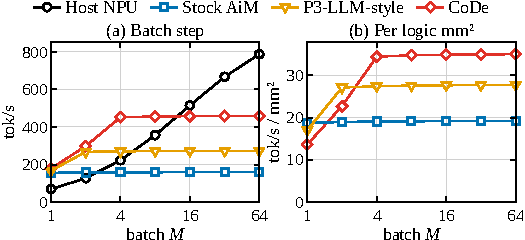
\includegraphics[width=\columnwidth]{figs/fig_hbm2.pdf}
  \caption{Edge server, batched decode step: (a)~tokens per second; (b)~tokens per second per logic mm$^2$.}
  \label{fig:hbm2}
\end{figure}

\subsection{Edge-Server Platform against P3-LLM-Style}
\label{sec:eval:server}

CoDe runs batched decode steps on HBM2 faster than P3-LLM-style, and the speed more than repays CoDe's larger logic;
Fig.~\ref{fig:hbm2} plots the geometric mean over the five LLMs at each batch.

\paragraph{Beats per command}
CoDe runs four beats per command where P3-LLM-style runs two. From batch 8 CoDe's step is 1.68$\times$
P3-LLM-style's and 2.87--2.88$\times$ stock AiM's; at batch 3--6 CoDe's step is 1.44--1.71$\times$ P3-LLM-style's
(Fig.~\ref{fig:hbm2}a). For one decoder layer's weight GEMMs of Llama-3.1-8B at batch 8, P3-LLM-style still issues one
command per token and fills 0.791 of the C bus, while CoDe fills 0.431 at about twice P3-LLM-style's useful-MAC
utilization ($U = 0.739$ against 0.379). CoDe's step stays ahead of the NPU up to batch 8--12, so a batch of 8, where P3-LLM~\cite{p3llm} moves its
linear layers to the NPU, still runs faster on CoDe.

\paragraph{Speed against area}
CoDe's speed more than pays for its larger logic. CoDe returns 1.26$\times$ P3-LLM-style's throughput per logic
mm$^2$ from batch 8 and 1.08--1.29$\times$ at batch 3--6 (Fig.~\ref{fig:hbm2}b). At batch 1--2, where CoDe's third and
fourth beats sit idle, P3-LLM-style's smaller PU leads (0.80--0.84$\times$).

\paragraph{System energy}
CoDe's speed lead carries over to system energy. From batch 8, P3-LLM-style spends 1.64$\times$ CoDe's system energy per token with P3-LLM's~\cite{p3llm} NPU idling at 55\,W
during PIM steps and 1.46$\times$ with the NPU power-gated, so CoDe's lead does not rest on the idle charge.

\paragraph{Sources of CoDe's gain}
CoDe's gain over stock AiM has two sources, and each source is worth more once the other is present. Both sources
come from one mechanism, the $V$ tokens that one tile MAC command serves: row reuse raises the sweep factor, and
beat filling raises the slot factor of Section~\ref{sec:bg:cmd}.
% sources-of-gain table (D-35): defined inside IV-C's last paragraph, past page 7's column break, so it renders at
% the top of the right column, opposite Fig. 6; generated by scripts/make_tables.py (simulated rows, evaluation/dac_2x2 Sec. 2i)
\begin{table}[t]
  \caption{Useful-MAC utilization from stock AiM to CoDe, one source at a time.}
  \label{tab:umac_src}
  \centering
  \footnotesize
  \setlength{\tabcolsep}{4pt}
  % generated by scripts/make_tables.py from evaluation/dac_2x2/figures/tab_umac_src_steps.csv (usrc_steps ids, simulated rows, layer, M = 8); do not edit
\begin{tabular}{@{}lccccc@{}}
\toprule
Design & \UMAC & \fMAC & $U$ & \multicolumn{2}{c@{}}{Speedup} \\
\cmidrule(l){5-6}
 & & & & step & cumul. \\
\midrule
\multicolumn{6}{@{}l}{\emph{Mobile:} Llama-2-7B, $V = 8$} \\
Stock AiM & 0.25 & 0.776 & 0.194 & -- & 1.00 \\
Row reuse only & 0.25 & 0.965 & 0.241 & 1.24 & 1.24 \\
\textbf{CoDe} & 1.00 & 0.843 & 0.843 & 3.49 & 4.35 \\
\midrule
\multicolumn{6}{@{}l}{\emph{Server:} Llama-3.1-8B, $V = 4$} \\
Stock AiM & 0.25 & 0.771 & 0.193 & -- & 1.00 \\
Row reuse only & 0.25 & 0.887 & 0.222 & 1.15 & 1.15 \\
\textbf{CoDe} & 1.00 & 0.739 & 0.739 & 3.33 & 3.83 \\
\bottomrule
\end{tabular}

\end{table}
Table~\ref{tab:umac_src} adds the two sources in that
order for one decoder layer's weight GEMMs at $M = 8$, the layer of Table~\ref{tab:umac} on the mobile platform and
of Llama-3.1-8B on the edge server. The row-reuse-only design keeps the stock PU's pace of one beat per column
period and adds CoDe's storage and row sweeps of $V$ tokens; we simulate it as CoDe's trace at $D = 1$ rather than compose it from the other rows. Row reuse alone lifts
\fMAC, yet $U$ reaches only 0.241 on the mobile platform and 0.222 on the edge server, because \UMAC stays at 1/4.
Beat filling, the command decoupling of Section~\ref{sec:design:beat}, then fills the idle beats and supplies the large step,
3.49$\times$ on the mobile platform and 3.33$\times$ on the edge server. In the other order, beat filling alone,
composed from the model, would reach a $U$ of only 0.464 and 0.506, in steps of 2.39$\times$ then 1.82$\times$ on the mobile
platform and 2.62$\times$ then 1.46$\times$ on the edge server, because the unchanged non-MAC commands would take
about half of the shortened time and \fMAC would fall. Beat filling thus earns its full step only once row reuse has
removed most of the row-switch overhead per token.

\subsection{Peak Power}
\label{sec:eval:power}

CoDe's faster PU clock leaves its peak power within a few percent of LP-Spec-style's on both platforms, so CoDe's peak
power stays at the level of the wider-PU design that LP-Spec~\cite{lpspec} proposes. With every PU at its full MAC
rate, CoDe draws 1.04$\times$ LP-Spec-style's peak power per die on the mobile platform and 1.03$\times$ per
pseudo-channel on HBM2 (Table~\ref{tab:params}). Stock AiM and P3-LLM-style draw less because they run fewer MACs per
column period.

\paragraph{Cost of the faster clock}
CoDe's 800\,MHz mobile clock itself costs little energy. Synthesised for 800\,MHz, the same 32-lane INT8 arithmetic
spends 2.4\,\% more energy per MAC than for 200\,MHz. The rest of CoDe's higher PU power comes from its clocked
storage: CoDe's staging registers and clock tree take the clock at four times LP-Spec-style's rate, even in cycles
where a register holds its value. LP-Spec-style pays in leakage instead: its PU, with four times CoDe's multipliers,
leaks 2.9$\times$ CoDe's power on the mobile platform and 2.8$\times$ on HBM2.

\paragraph{Charge per clock edge}
CoDe spreads the same MAC rate over four times as many clock edges, so each edge draws far less charge. CoDe's PUs
switch 522\,pJ per die every 1.25\,ns against LP-Spec-style's 1,776\,pJ every 5\,ns, so each CoDe edge draws
3.4$\times$ less charge from the supply; on HBM2 the ratio is 3.1$\times$. A smaller charge per edge lowers the
current step that the die's power grid absorbs.

\paragraph{Clock gating in CoDe}
CoDe's registers sit idle on most cycles, so clock gating cuts CoDe's power far more than LP-Spec-style's. Each of
CoDe's accumulator slots takes one write every 16 cycles, and each staging word takes one every 6 cycles on the mobile
platform and every 8 on HBM2, while LP-Spec-style's mobile PU writes every register on every cycle. A clock gate on
each accumulator slot, on each 32 bits of a staging word and on the weight latch cuts CoDe's peak power by 11.6\,\% on
the mobile platform and 15.1\,\% on HBM2, against 0.5\,\% and 3.6\,\% for the same gates on LP-Spec-style's
accumulators and staging words. Gated CoDe then draws 0.92$\times$ ungated LP-Spec-style's peak power on the mobile
platform and 0.87$\times$ on HBM2. Gating remains an option: every other number in this paper describes the ungated
designs.
